\section{\ttt{3D} Classification and Refinement}

 \begin{figure}[H]
  \centering
  \captionsetup{width=.8\linewidth} 
  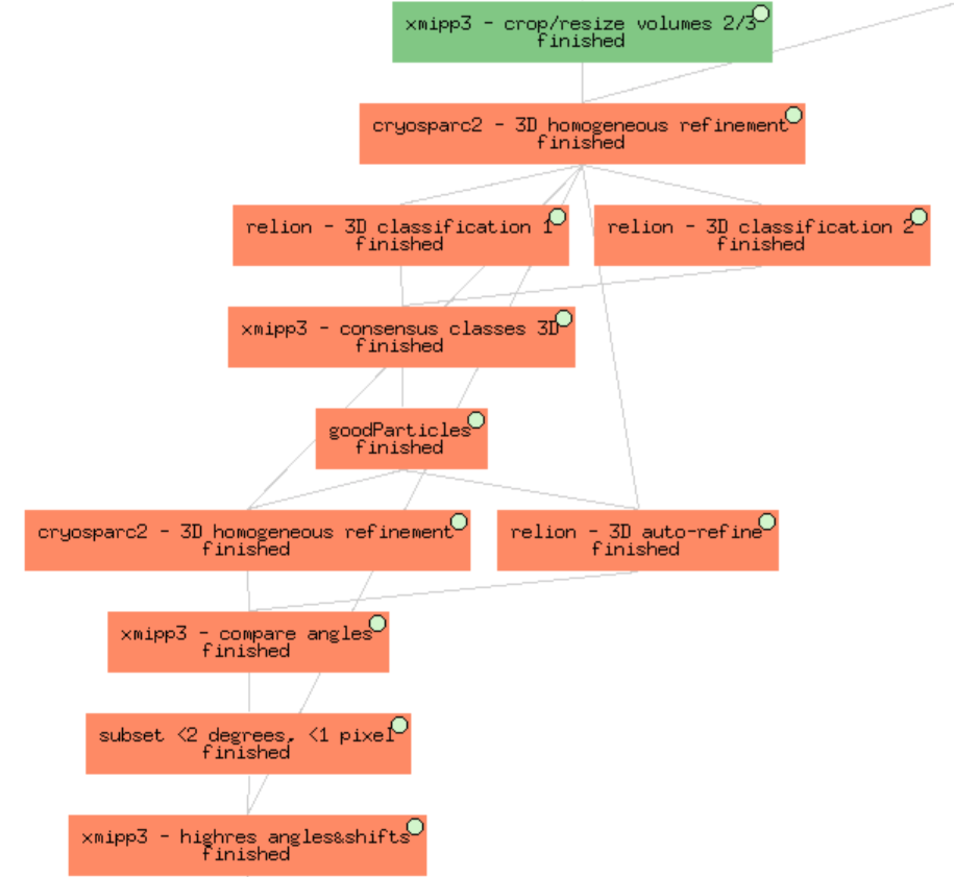
\includegraphics[width=1\textwidth]
  {{images/9_workflow7_3D_RandC.pdf}}
  \caption{Refinement and \ttt{3D} Classification.}
  \label{fig:workflow_7}
  \end{figure}

\ttt{3D} Classification and Refinement are the two last overlapping steps in image processing. They consume the most time and resources with the aim of obtaining a \ttt{3D} map at the highest possible resolution. This is only feasible if data is homogeneous enough, $i.e.$, if data represent a unique conformation of the specimen.\\

\subsection*{Refinement of the initial map}
Before starting with the \ttt{3D} classification properly, a refinement step will be performed with our initial map. The first approach to get a high resolution map in a fully automated manner was performed with the algorithm $Cryosparc$ \ttt{homogenous refinement}. This procedure rapidly refines a single homogeneous structure to high-resolution and validate using the gold-standard Fourier Shell Correlation (FSC). We have implemented it in the protocol \scommand{cryosparc2-homogeneous refinement} (\ffigure{fig:cryosparc_refine}). In the \ttt{Input} tap of this protocol form we include the subset of homogeneous particles extracted previously and the initial volume computed, as well in the \ttt{Refinement} tap we will choose the symmetry (octahedral), we will select all the options and we will choose in \ttt{Noise model} symmetric. 

\begin{figure}[H]
  \centering
  \captionsetup{width=.8\linewidth} 
  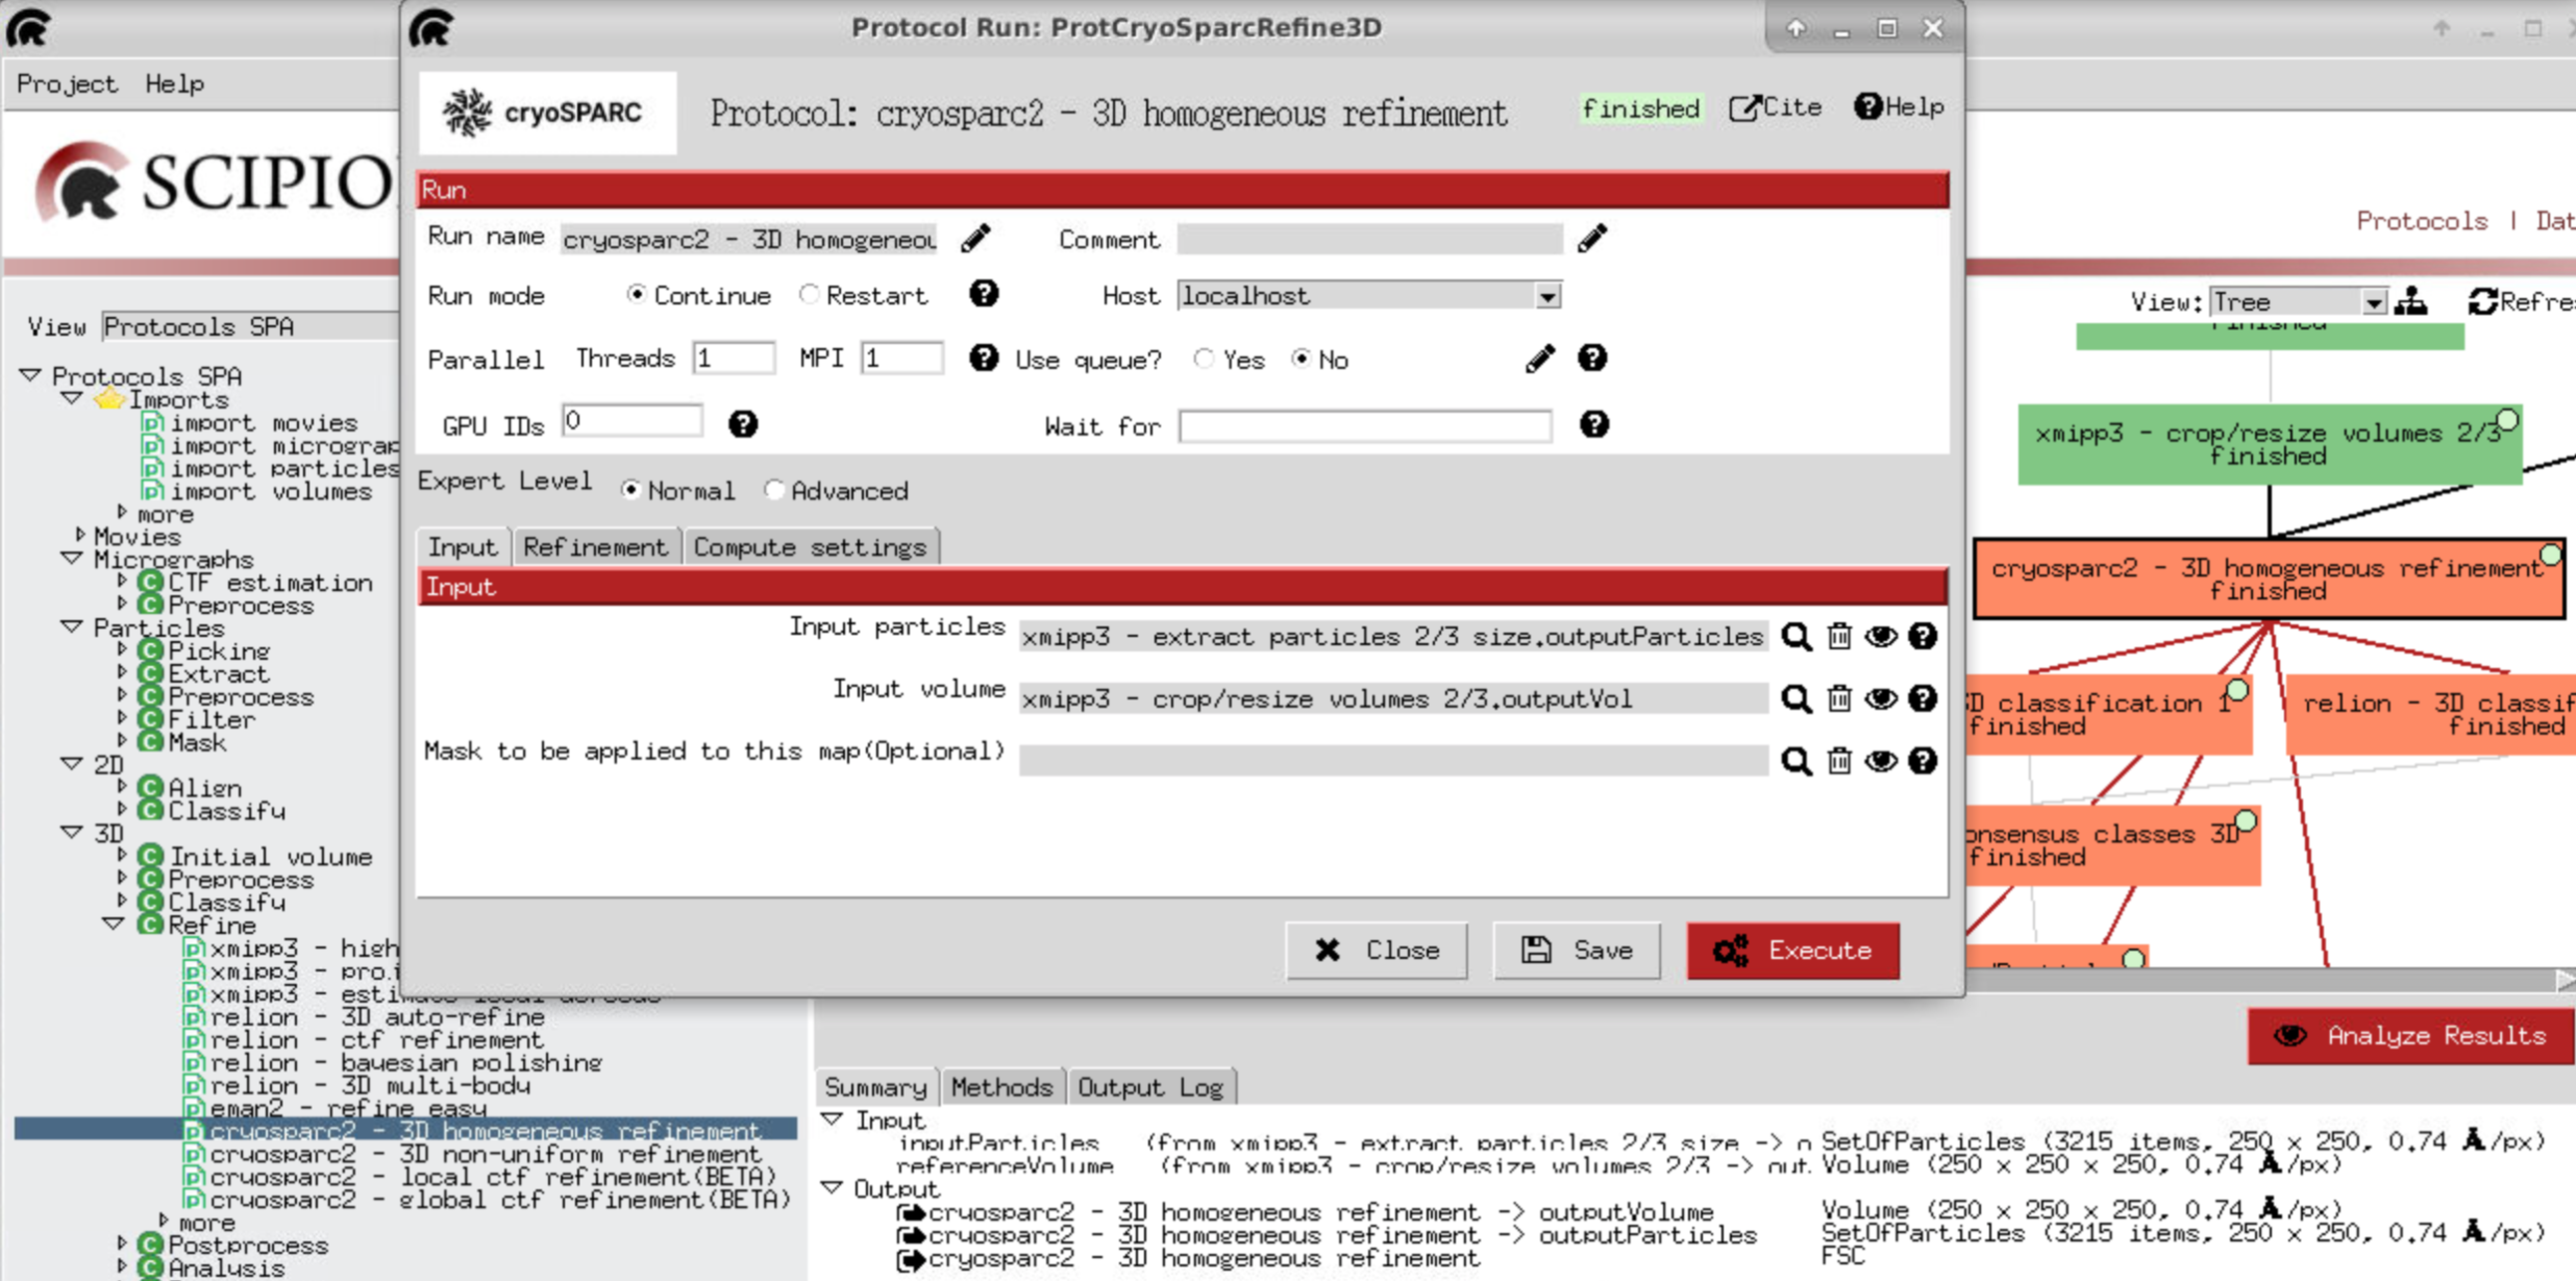
\includegraphics[width=0.95\textwidth]
  {{images/9a_cryosparc2_3Dhrefinement.pdf}}
  \caption{Completing the params of the protocol \scommand{cryosparc2-homogeneous refinement}.}
  \label{fig:cryosparc_refine}
  \end{figure}

After executing, a refined map of 3.3 \AA\ of final resolution was obtained as output, with the same size and sampling rate that we had in the inputs. Press \scommand{Analyze Results} to visualize the FSC, the volume or the set of particles. With our initial volume and set of particles we can see that it nicely converge in a good 3D structure, however, we do not know if all the particles that we have used are consistent with that structure and we also do not know if the parameters of those have been correctly identified. These would be tried to be solved in the next section.

\subsection*{3D classification}
To continue with the refinement process to obtain a better resolution and to answer the first question, if all the particles belong to that structure, we start executing two independent times the same algorithm of $Relion$ \ttt{3D classification} that we have implemented in the protocol \scommand{relion-3D classification} (\ffigure{fig:relion_3Dclassification}). In the tap \ttt{Input} we include the particles derived from executing the previous protocol \scommand{cryosparc2-homogeneous refinement}. The volume derived from this protocol will be the \ttt{Input volume(s)} in the tap \ttt{Reference 3D map} and will be low-pass filtered by 15\AA\. The optimization params appear in the tap \ttt{Optimization}: 2 \ttt{Number of classes} and 25 \ttt{Number of iterations}. As \ttt{Regularisation parameter T} values as 3-4 are common for \ttt{3D} classification.

\begin{figure}[H]
  \centering
  \captionsetup{width=.8\linewidth} 
  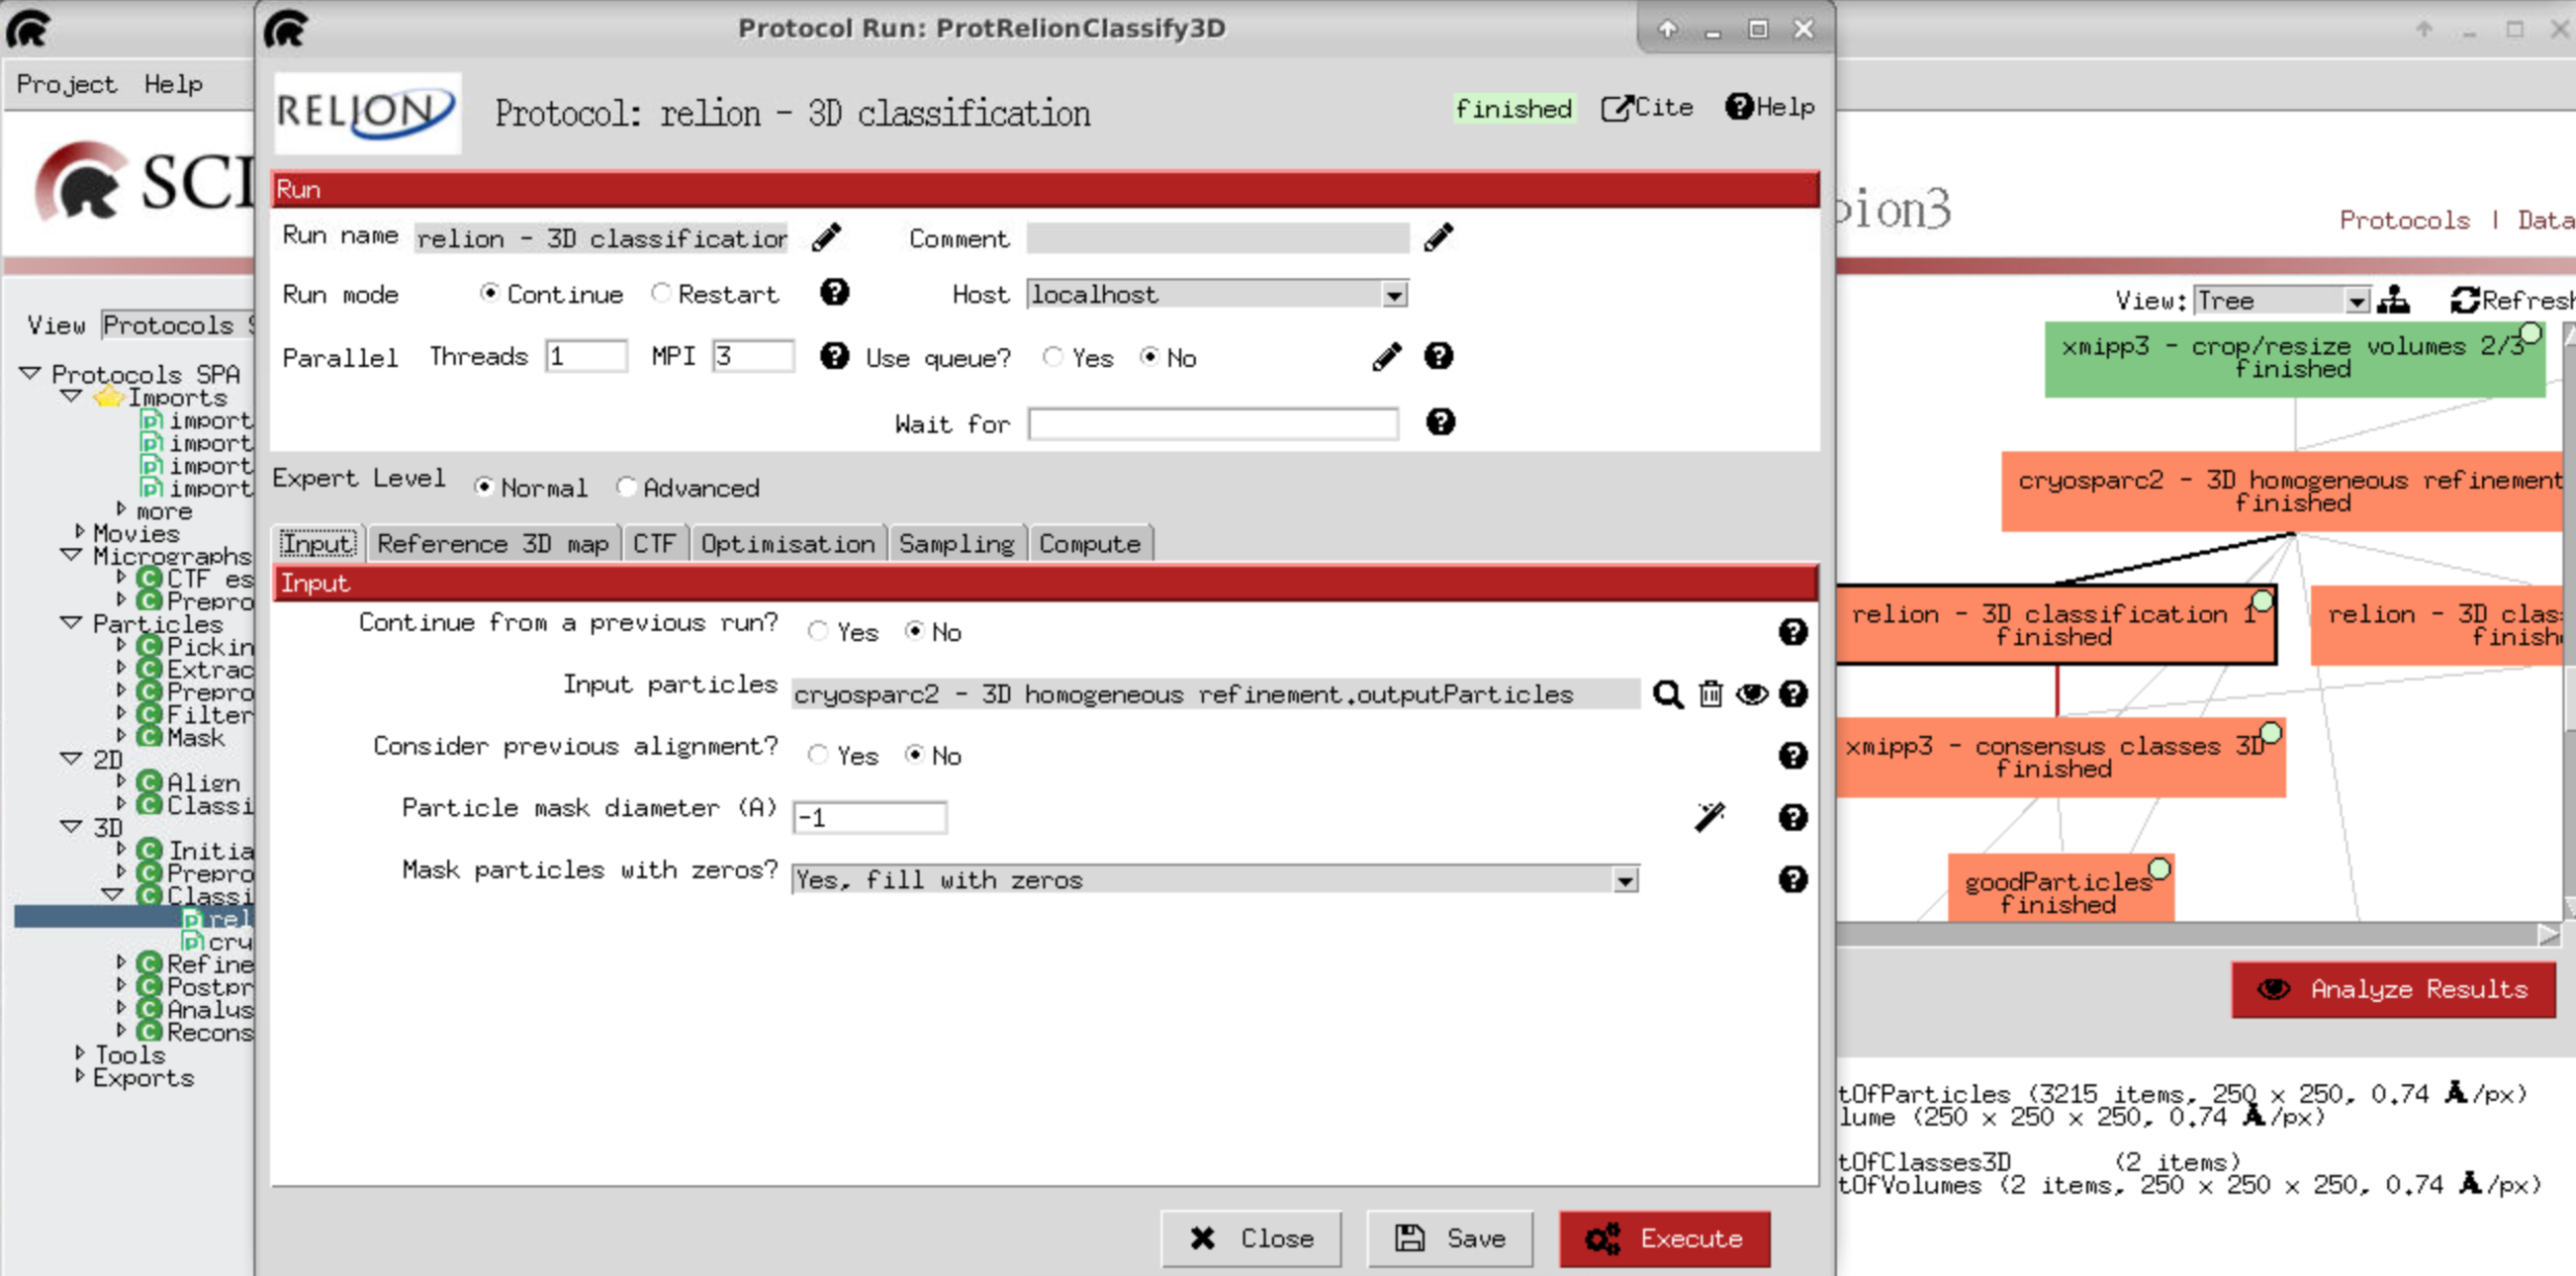
\includegraphics[width=0.95\textwidth]
  {{images/9b_relion_3DClassf_1.pdf}}
  \caption{Completing the params of the protocol \scommand{relion-3D classification}.}
  \label{fig:relion_3Dclassification}
  \end{figure}
  
The output of each one of these two \scommand{relion-3D classification} protocols are 2 maps with the initial size and sampling rate, reconstructed from different groups of reclassified particles. By pressing \scommand{Analyze Results} and \ttt{Particles/ Show classification in Scipion}, a table will be opened showing the projection representative of each map and the number of particles contributing to its reconstruction:
\begin{itemize}
 \item 2428 and 787 in the first classification.
 \item 2460 and 755 in the second one.
\end{itemize}

The results of the first and second \ttt{3D} classifications are similar, in both cases the first class contains most of the particles. In order to have a consensus of these results, we execute the protocol \scommand{xmipp3-consensus classes 3D} that compares several sets of \ttt{3D} classes and return the intersection of the input classes (\ffigure{fig:consensus_classes}).

\begin{figure}[H]
  \centering
  \captionsetup{width=.8\linewidth} 
  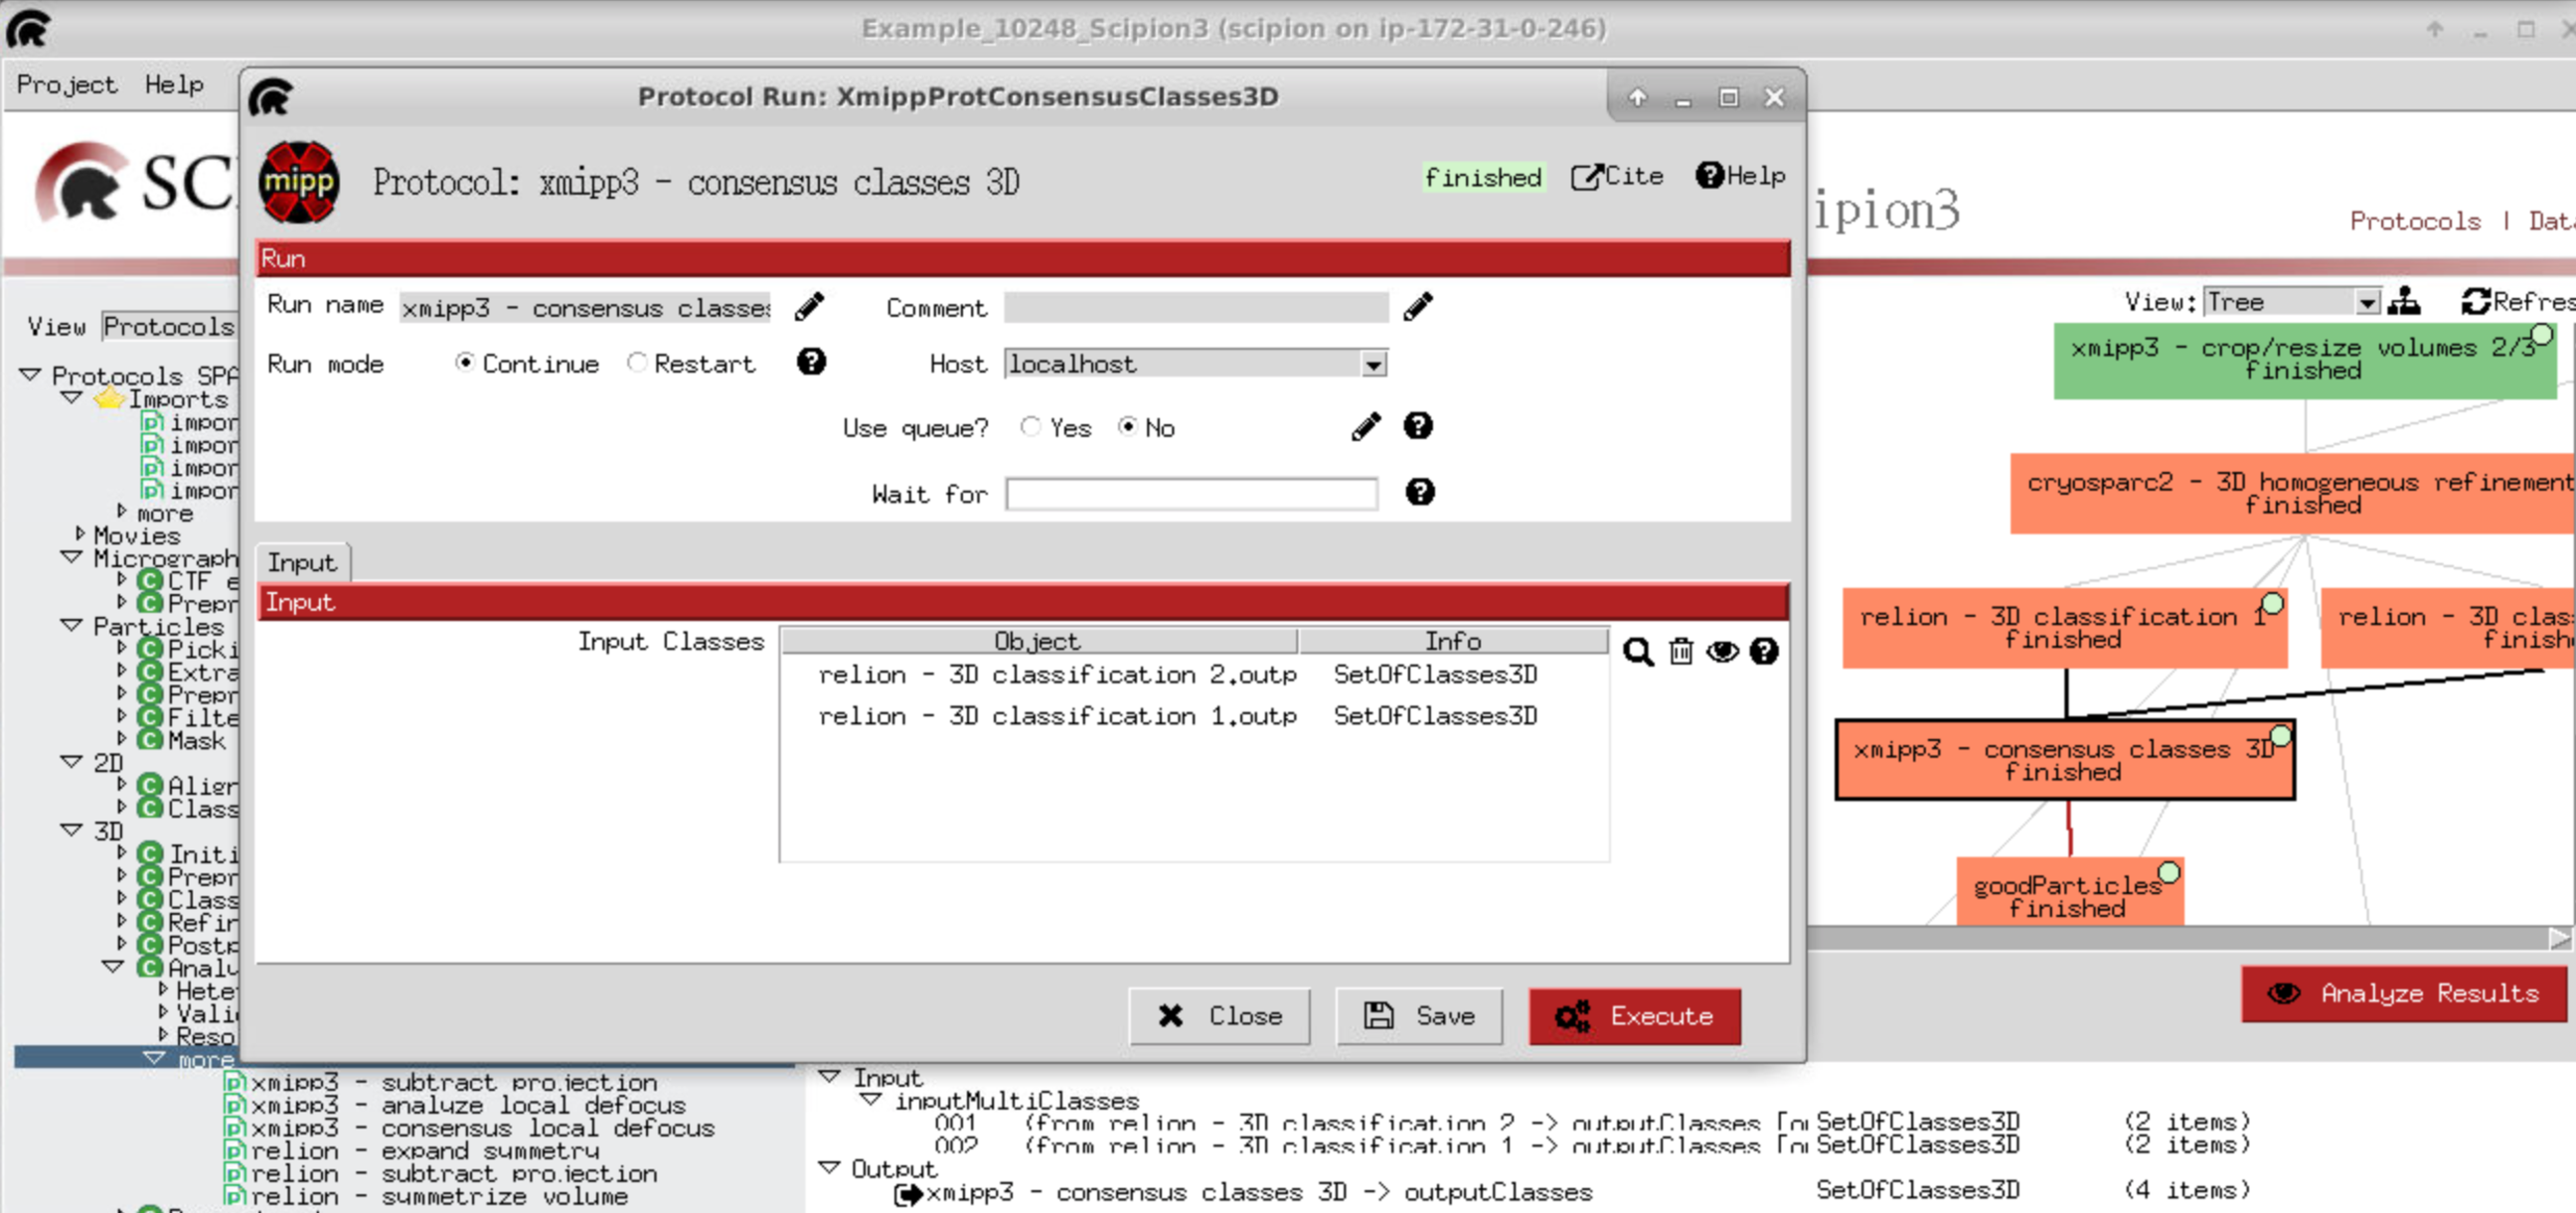
\includegraphics[width=0.95\textwidth]
  {{images/9d_xmipp3_3Dconsensus.pdf}}
  \caption{Filling in the params of the protocol \scommand{xmipp3-consensus classes 3D}.}
  \label{fig:consensus_classes}
  \end{figure}
  
By pressing \scommand{Analysis Results} you can visualize the 4 intersection \ttt{3D} classes with the number of particles assigned to each one. The first of these classes derive from about 1944 particles (aprox. 60\% of total particles). Once inspected the different classes, by selecting the classes that we are interested in (only the first one) and pressing \scommand{Particles}, a new set of 1944 particles will be created included in the box \ttt{goodParticles}.\\

\subsection*{Final refinement iterations with $Xmipp$ \ttt{highres}}
 \begin{figure}[H]
  \centering
  \captionsetup{width=.8\linewidth} 
  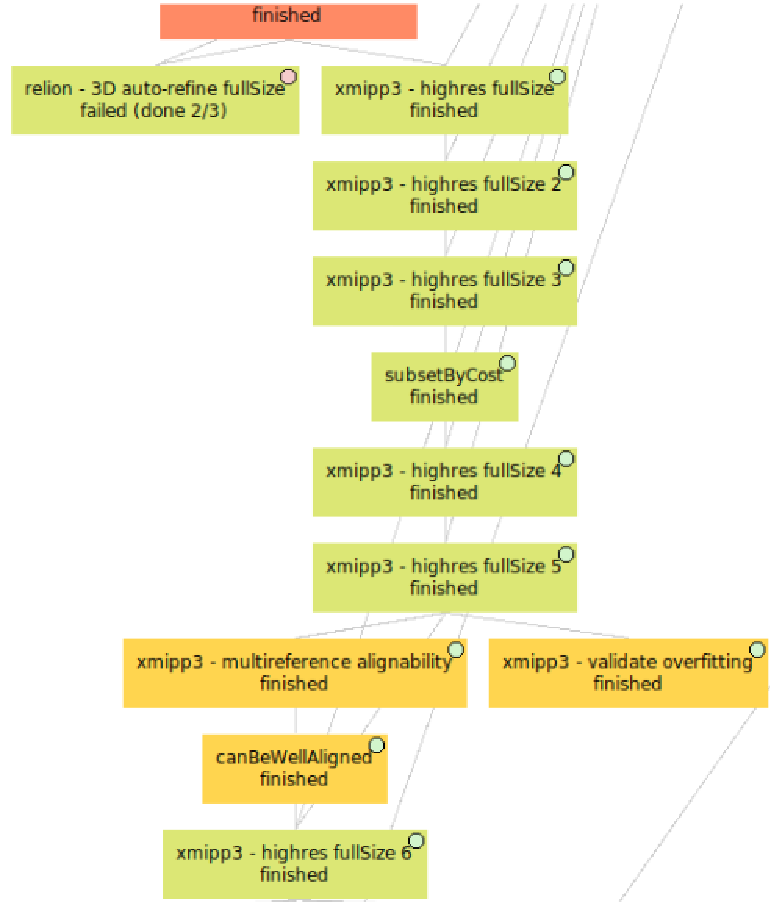
\includegraphics[width=0.7\textwidth]
  {{images/workflow_8.pdf}}
  \caption{Map final refinement (Light green color).}
  \label{fig:workflow_8}
  \end{figure}
  
From now ahead several steps of refinement will be accomplished using the above mentioned protocol \scommand{xmipp3-highres}. The input of the first round of refinement includes the particles extracted with the previous protocol and the volume generated by the same algorithm before performing the \ttt{3D} classification step (\ffigure{fig:highres_fullsize}). In the \ttt{Angular assignment} tap, we select \ttt{Global} for the \ttt{Image alignment} param, 1 as \ttt{Number of iterations} and 3 as \ttt{Max. Target Resolution}.

 \begin{figure}[H]
  \centering
  \captionsetup{width=.8\linewidth} 
  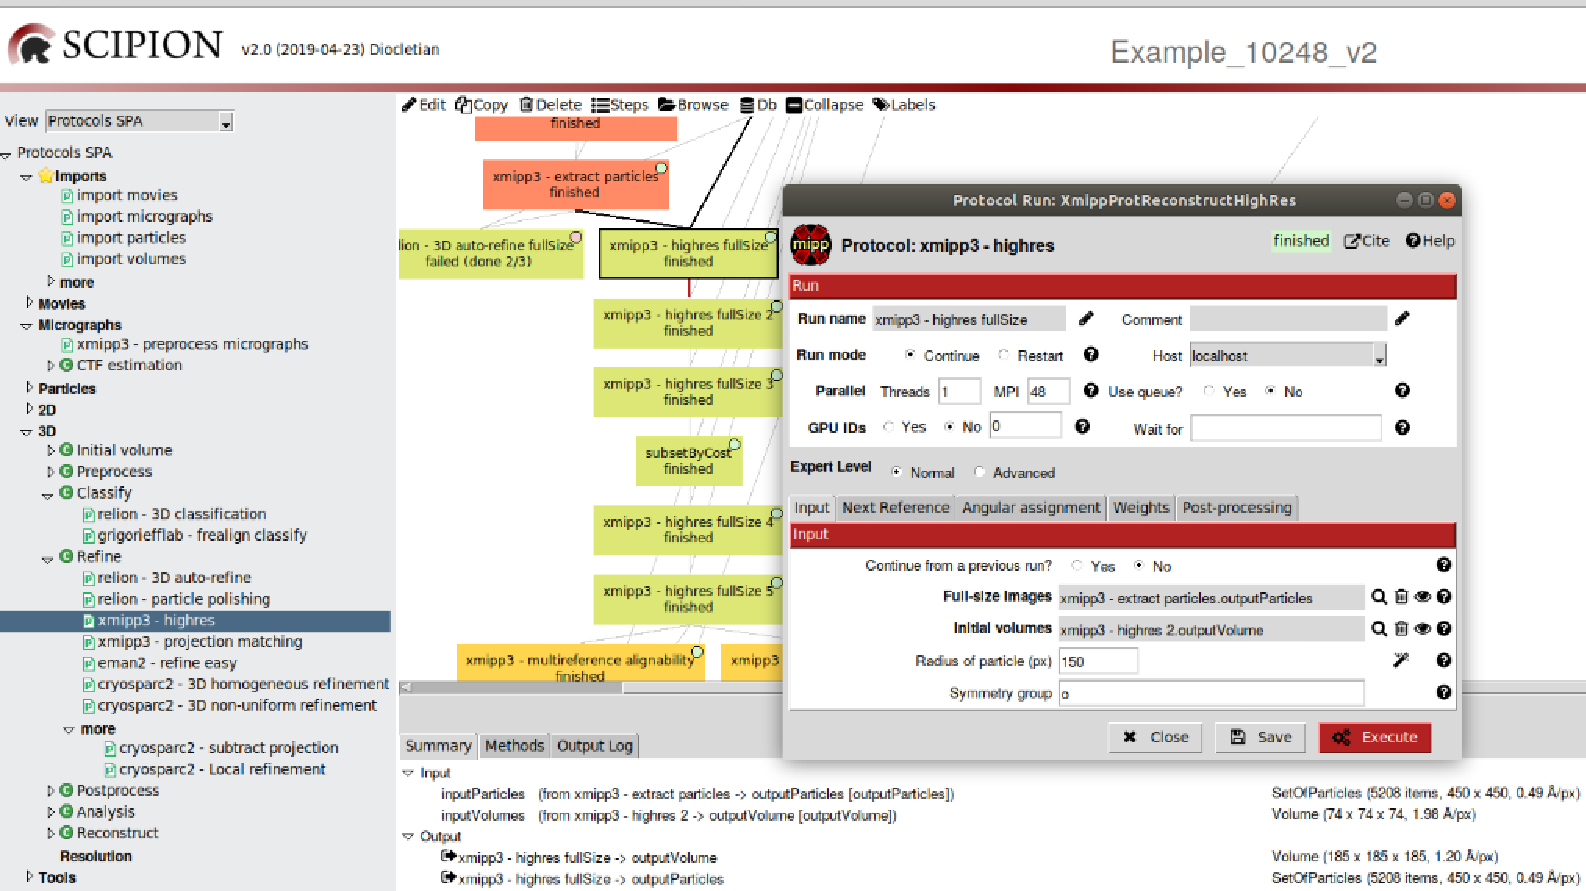
\includegraphics[width=0.95\textwidth]
  {{images/highres_fullsize.pdf}}
  \caption{$Xmipp$ \ttt{highres} map global refinement (Iteration 1).}
  \label{fig:highres_fullsize}
  \end{figure}
  
The output resampled volume generated can be seen by pressing \scommand{Analyze results}, as well as the particles from which it derives.\\

The second run of refinement continues from the previous one, as it is selected in the \ttt{Input} tap. The particles derived from the first round of refinement are included as input params. The same params have been selected in the \ttt{Angular assignment} tap (\ffigure{fig:highres_fullsize2}).

 \begin{figure}[H]
  \centering
  \captionsetup{width=.8\linewidth} 
  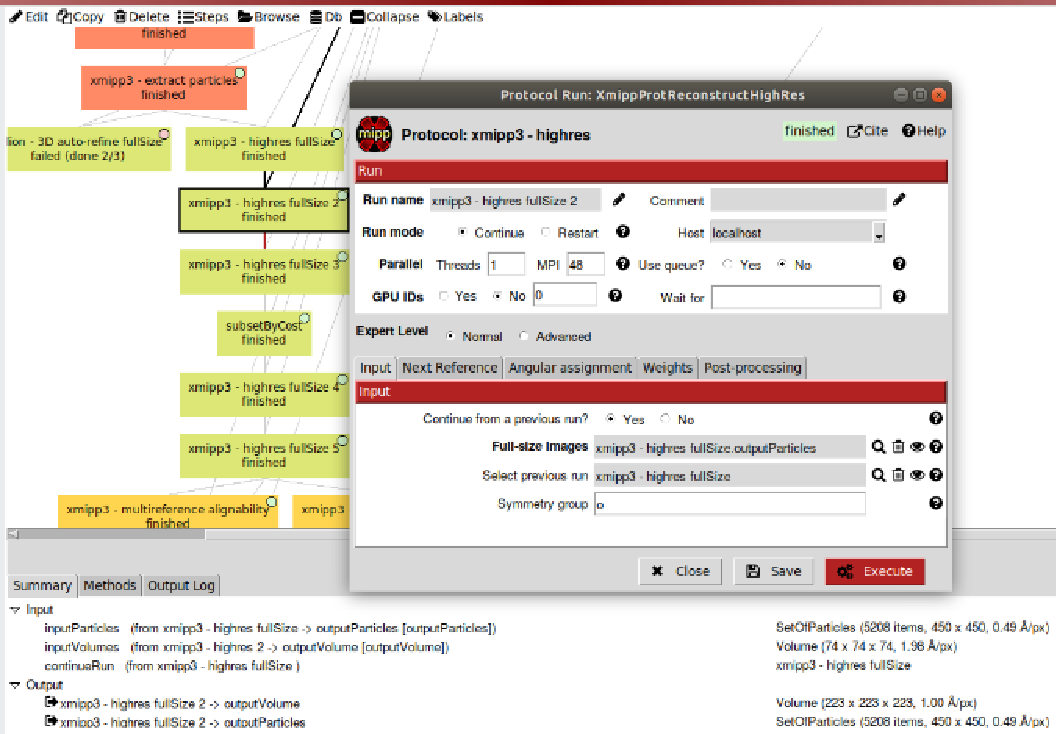
\includegraphics[width=0.95\textwidth]
  {{images/highres_fullsize2.pdf}}
  \caption{$Xmipp$ \ttt{highres} map global refinement (Iteration 2).}
  \label{fig:highres_fullsize2}
  \end{figure}

A new output resampled volume has been obtained that move from 1.20 \AA/px to 1.00 \AA/px).\\

Once we have finished the global refinement, we continue with the local refinement in the third round of refinement (\ffigure{fig:highres_fullsize3}). Again, we use the particles derived from the previous iteration. In this case, we select \ttt{Local} for the \ttt{Image alignment} param and 2.5 for the \ttt{Max. Target Resolution} of tap \ttt{Angular assignment}. \ttt{Shifts} and \ttt{angles} will be also optimized.

 \begin{figure}[H]
  \centering
  \captionsetup{width=.8\linewidth} 
  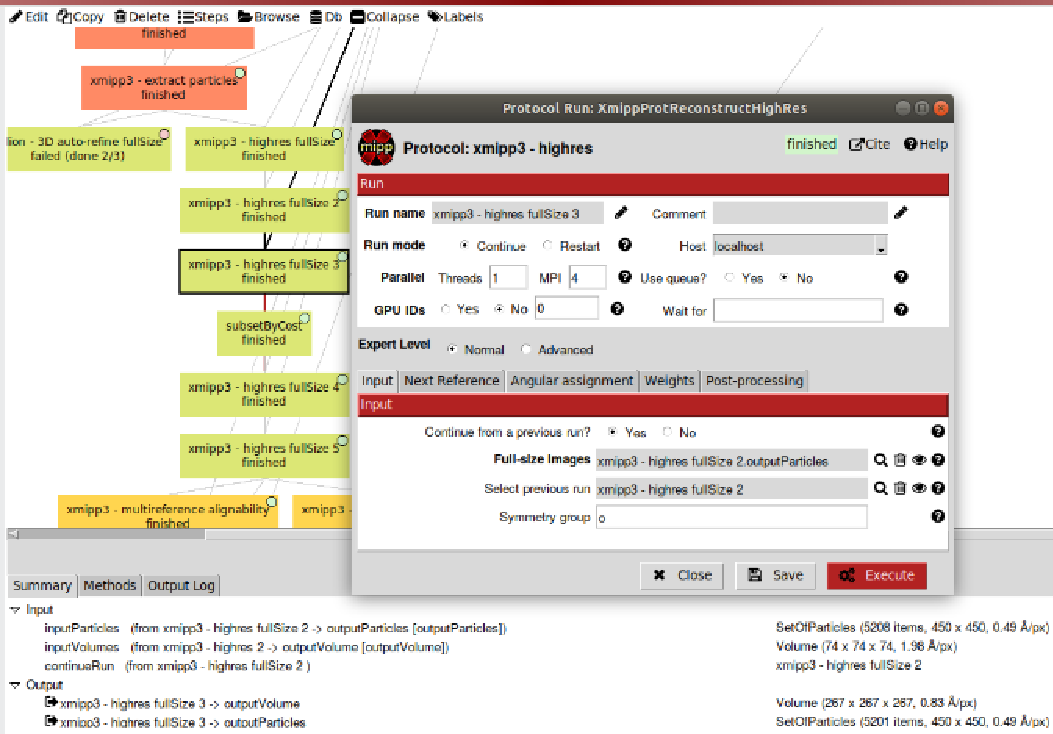
\includegraphics[width=0.95\textwidth]
  {{images/highres_fullsize3.pdf}}
  \caption{$Xmipp$ \ttt{highres} map local refinement (Iteration 3).}
  \label{fig:highres_fullsize3}
  \end{figure}

The output resampled volume obtained (0.83 \AA/px) derives from a set of particles slightly smaller (5,201). The table of particles can be also observed by pressing \scommand{Analyze results}. We can select particles according to the value of the \ttt{\_xmipp\_cost} param. Choosing values higher than 0.15, a total of 696 particles (13.4\%) of the input set has been removed. The remaining 4,505 particles will be used as inputs of the fourth round of refinement (\ffigure{fig:highres_fullsize4}). Params from \ttt{Angular assignment} tap will remain unchanged except the \ttt{Optimization} ones. In addition to \ttt{shifts} and \ttt{angles}, \ttt{scale} and \ttt{defocus} will be also optimized.

\begin{figure}[H]
  \centering
  \captionsetup{width=.8\linewidth} 
  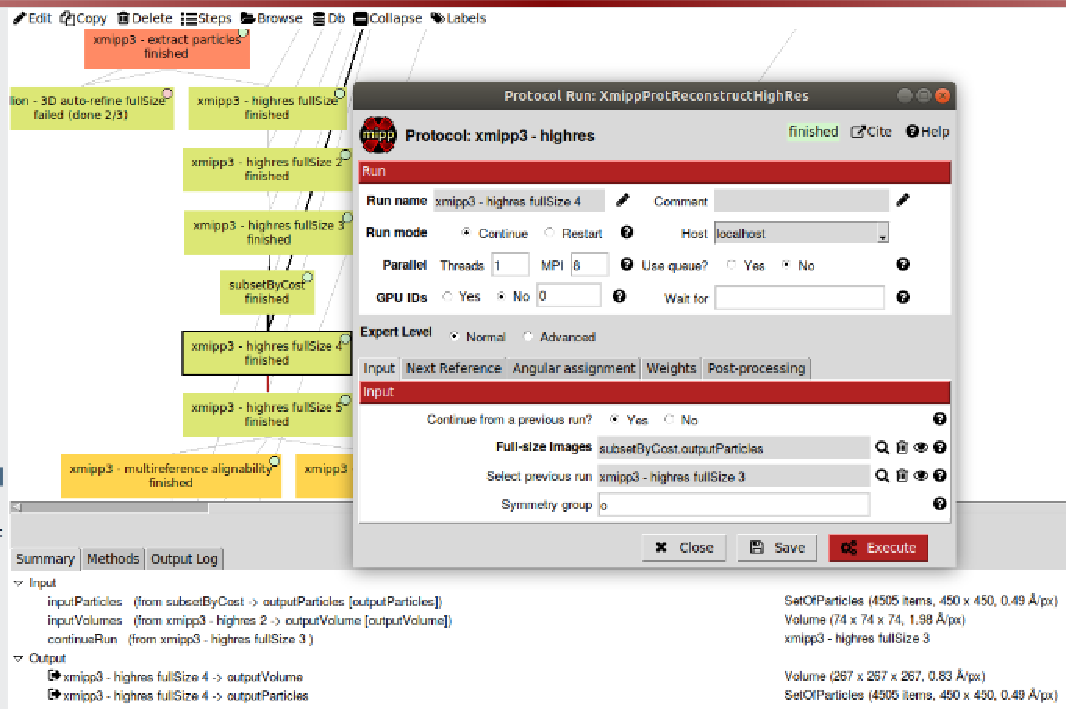
\includegraphics[width=0.95\textwidth]
  {{images/highres_fullsize4.pdf}}
  \caption{$Xmipp$ \ttt{highres} map local refinement (Iteration 4).}
  \label{fig:highres_fullsize4}
  \end{figure}
  
The new map, based on the last set of particles, appears in the output. These particles are included in the input of the fifth round of local refinement (\ffigure{fig:highres_fullsize5}). This time, we reduce the value of the \ttt{Max. Target Resolution} param to 2.25 and set to \ttt{Yes} all the \ttt{Optimization} params.

\begin{figure}[H]
  \centering
  \captionsetup{width=.8\linewidth} 
  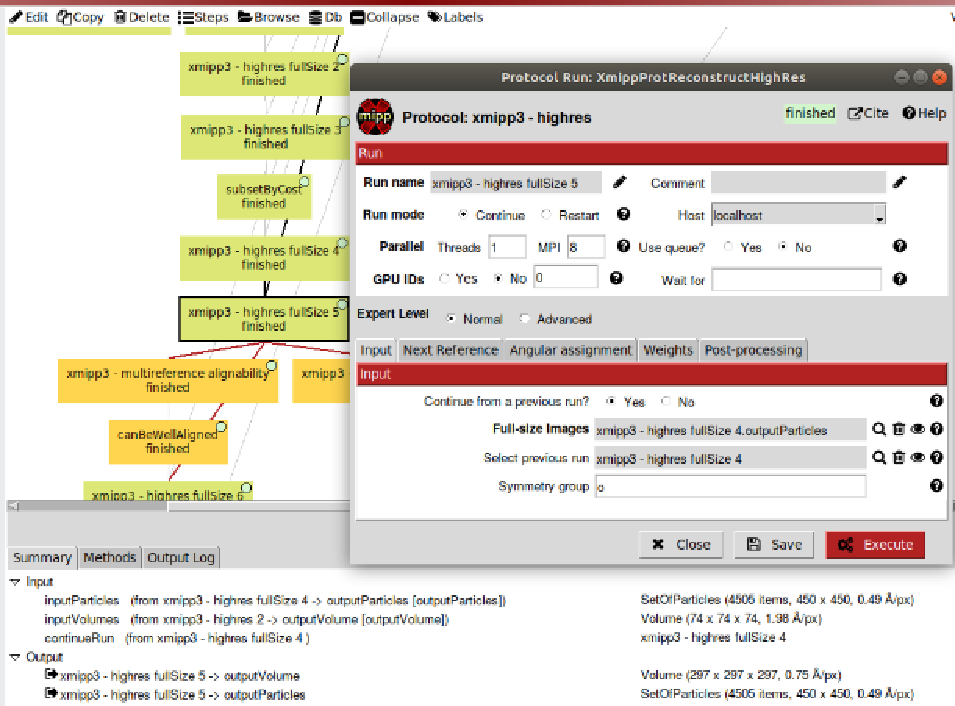
\includegraphics[width=0.95\textwidth]
  {{images/highres_fullsize5.pdf}}
  \caption{$Xmipp$ \ttt{highres} map local refinement (Iteration 5).}
  \label{fig:highres_fullsize5}
  \end{figure}
  
Before continuing with the sixth round of refinement we are going to assess the output resampled map (0.75\AA/px) regarding soft alignability and overfitting of particles and \ttt{3D} map. Two protocols are going to be independently executed: \scommand{xmipp3-multireference alignability} (\ffigure{fig:multireference_alignability}) and \scommand{xmipp3-validate overfitting} (\ffigure{fig:validate_overfitting}). The input of both protocols requires map and particles generated in the last refinement iteration. 

\begin{figure}[H]
  \centering
  \captionsetup{width=.8\linewidth} 
  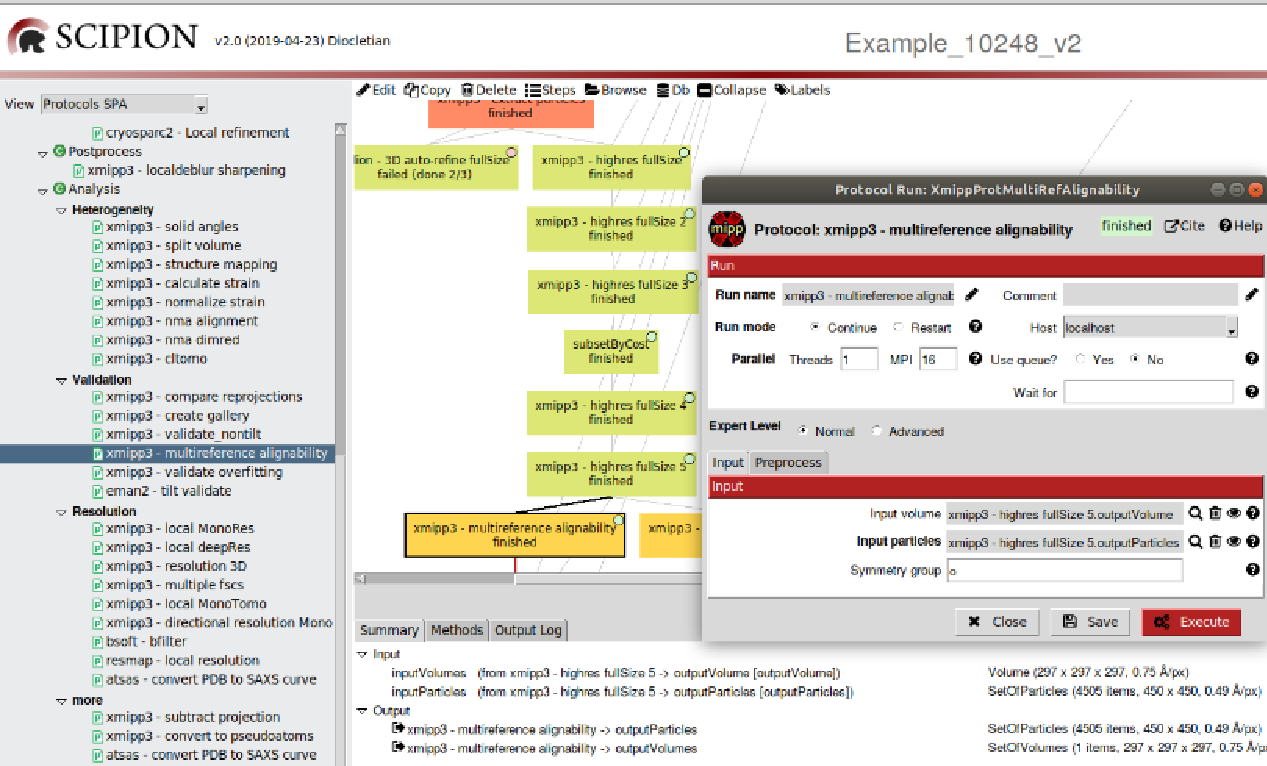
\includegraphics[width=0.95\textwidth]
  {{images/multireference_alignability.pdf}}
  \caption{Completing the form of the protocol \scommand{xmipp3-multireference alignability}.}
  \label{fig:multireference_alignability}
  \end{figure}
  
\begin{figure}[H]
  \centering
  \captionsetup{width=.8\linewidth} 
  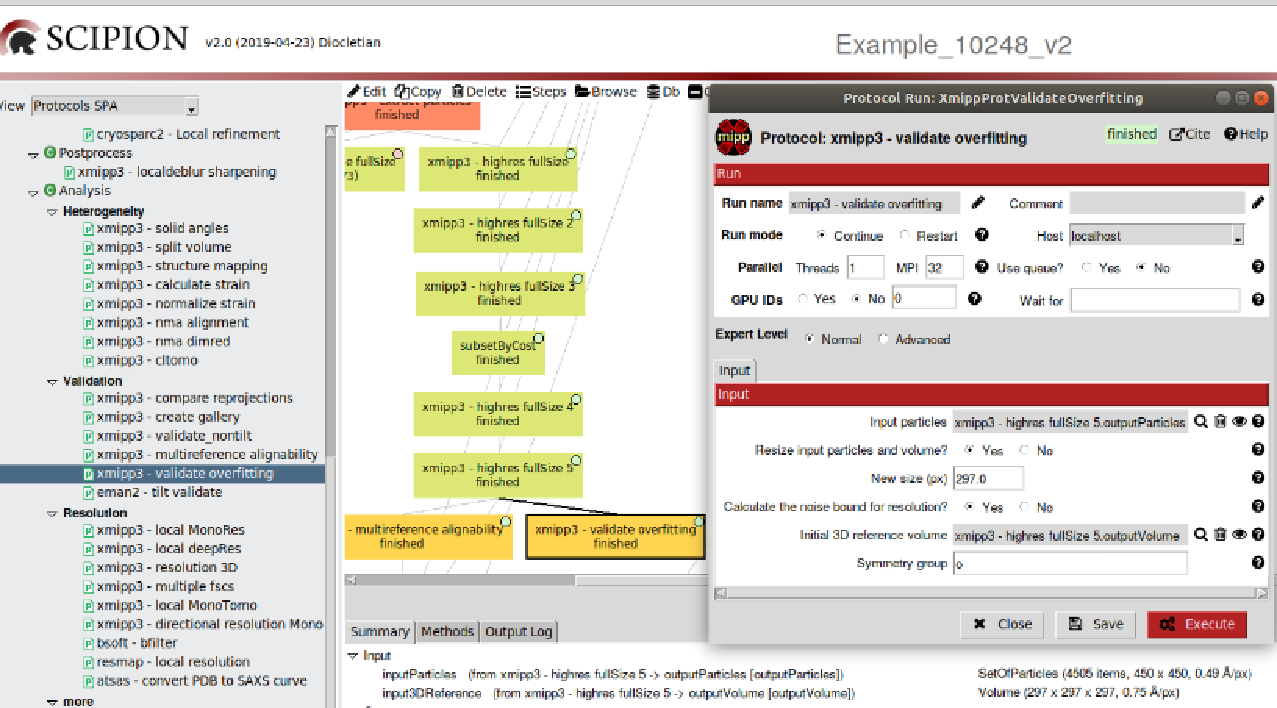
\includegraphics[width=0.95\textwidth]
  {{images/validate_overfitting.pdf}}
  \caption{Filling in the form of the protocol \scommand{xmipp3-validate overfitting}.}
  \label{fig:validate_overfitting}
  \end{figure}

The output values of particle alignment, precision and accuracy, generated by \scommand{xmipp3-multireference alignability} (press \scommand{Analyze Results} to check table columns \ttt{\_xmipp\_scoreAlignabilityAccuracy} and \ttt{\_xmipp\_scoreAlignabilityPrecission}) allow us to discard particles with worse alignment. In this case, 1,020 particles (22.6\% of the total input) are rejected. In order to improve the refined map resolution, the remaining 3,485 particles will be used to perform the sixth local refinement iteration with $Xmipp$ \ttt{highres} algorithm. The protocol params will remain unchanged compared with the fifth iteration.

\begin{figure}[H]
  \centering
  \captionsetup{width=.8\linewidth} 
  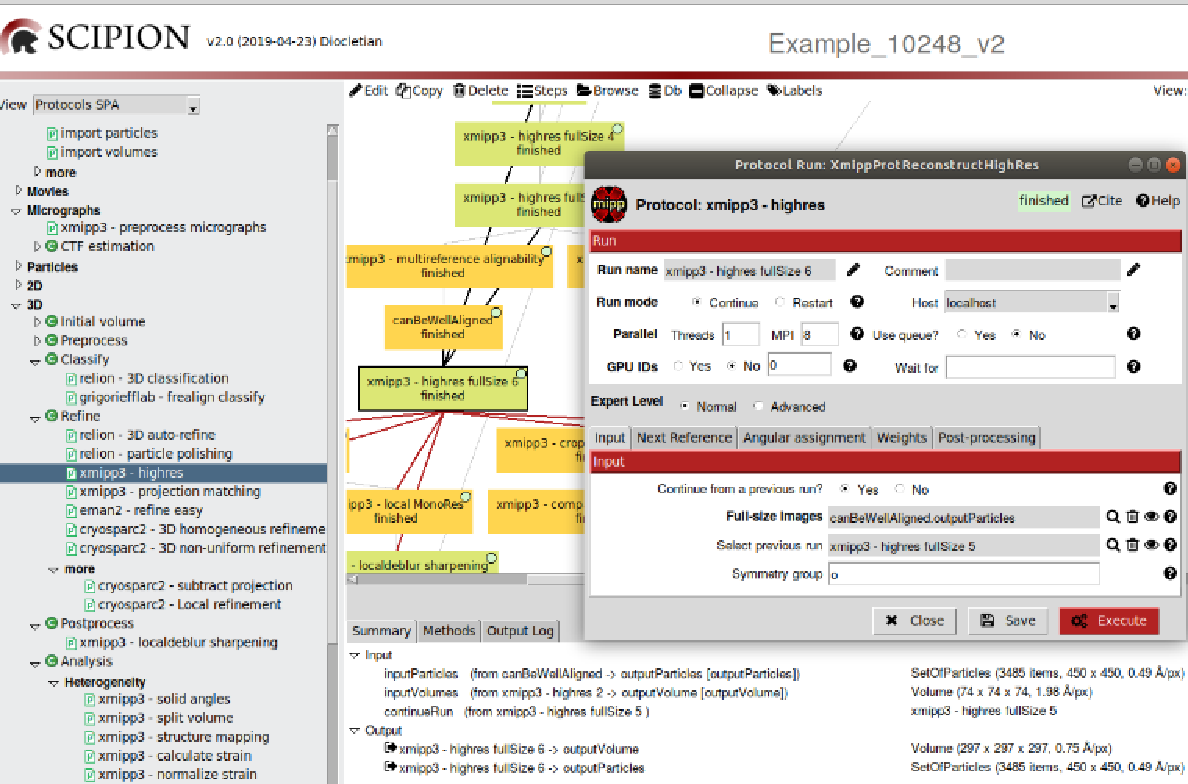
\includegraphics[width=0.95\textwidth]
  {{images/highres_fullsize6.pdf}}
  \caption{$Xmipp$ \ttt{highres} map local refinement (Iteration 6).}
  \label{fig:highres_fullsize6}
  \end{figure}

The sampling of the output map is the same than in the previous iteration, despite the selection of best aligned particles. We have thus achieved convergence and we can compute the global or local resolution. The local resolution can be calculated with the protocol \scommand{xmipp3-local MonoRes} \citep{vilas2018monores}. To have an overview of protocol and function of \ttt{MonoRes} see our \scipion tutorial in Model Building (download from \url{https://github.com/I2PC/scipion/wiki/tutorials/tutorial_model_building_basic.pdf}).       

  For more information: 
\begin{itemize}
   \item \textbf{Video tutorial}:  \url{https://www.youtube.com/watch?v=ial95OZJXU0&list=PLQjWIcrmtc4JjyC-_BM99_XW-VsDa4_i3&index=29}.
   \item \textbf{Theoretical lecture}:  \url{https://www.youtube.com/watch?v=taCREkFAPoE&list=PLQjWIcrmtc4JjyC-_BM99_XW-VsDa4_i3&index=36}.
  \end{itemize}            
